\documentclass{l4proj}

\usepackage{csquotes}
\usepackage[
backend=biber,
style=ieee
]{biblatex}
\addbibresource{bibliography.bib}

\begin{document}
\title{Building Applications on the SAFE Network}	
\author{David Brown}
\maketitle

\begin{abstract}
Lorem ipsum dolor sit amet, consectetur adipiscing elit, sed do eiusmod tempor incididunt ut labore et dolore magna aliqua. Ut enim ad minim veniam, quis nostrud exercitation ullamco laboris nisi ut aliquip ex ea commodo consequat. Duis aute irure dolor in reprehenderit in voluptate velit esse cillum dolore eu fugiat nulla pariatur. Excepteur sint occaecat cupidatat non proident, sunt in culpa qui officia deserunt mollit anim id est laborum.
\end{abstract}

\educationalconsent

\tableofcontents

\chapter{Introduction}
\pagenumbering{arabic}

\begin{displayquote}
The SAFE Network is a decentralized data storage and communications network that provides a secure, efficient
and low-cost infrastructure for everyone \cite{safenetwork}.
\end{displayquote}

The SAFE Network \cite{safenetwork} is an open-source project being developed by a Scottish company Maidsafe \cite{maidsafe}. Their aim is to build "The World's First Autonomous Data Network". An 'Autonomous Data Network' in simple terms, is "...a network that manages all our data and communications without any human intervention and without intermediaries" \cite{autonomous-data-networks}. This network will be decentralised, splitting data and then storing it around the world on computers called 'vaults'. I will go into more detail on the SAFE Network and how it works in \textit{Chapter \ref{ch:architecture}}.

\section{Aims}

My main goal for this project is to explore the usage of the SAFE Network for the purposes of providing decentralised and 'permissionless' access to websites like Wikipedia.

The program I build will be able to upload ZIM\cite{zim} files to the SAFE Network, provide public links to everyone using the application and then be able to read/browse the files. These files will be immutable, this is to help ensure that once a user has uploaded a ZIM file to the network, that it cannot be altered by anyone once it has been uploaded (apart from the functionality to delete it). ZIM files are a convenient way of being able to package/archive a website (web content) into an offline file that can then be browsed and distributed easily.

By building this application, it will be easy to draw conclusions on whether this method of 'archiving' websites to the SAFE Network is sensible. ZIM files themselves can easily be tens of gigabytes in size. Thus in building this program it will be feasible to ascertain how well the SAFE Network can handle large files.

\section{Motivation}

In my opinion, the right to liberty and the unobstructed access to information is the most important right we have. Throughout history, a common tactic of \textit{evil} governments or people is to block access to information. By doing this, they try to break down a culture, to control people. The most prominent example of this was the Nazi Book Burning Campaign \cite{book-burning}. The goal of this was to destroy any literature or information that could subvert the ideologies that Nazism is built upon.

The SAFE Network is an 'internet' which is impossible to block or orchestrate what content can be accessed without blocking access to the entire thing. A network that is built from the ground up to protect the free access to data, working autonomously and without judgement on what information is being stored and shared. By hosting archives/copies of websites such as Wikipedia and Wikispecies on the SAFE Network, it could allow people from all over the world to access content that they haven't before. More importantly for some people, for them to be able to access the content without their governments being able to detect what they are looking at.

\chapter{The SAFE Network}

Decentralisation of data is the core benefit of the SAFE Network. As with many things in life, once someone has ownership or control of something they can either use that position of power for good purposes or for less desirable ones. The internet as it exists today is very fragile in this regard. When you upload a file to Dropbox or OneDrive, where does this file exist? Well that file exists solely on the servers that those organisations have control over. Once an organisation has data they can do with it what they please, acting within the bounds of overcomplicated privacy polices to manage your data. Not only does this incur the obvious privacy infringements (which we will not cover cover too much within this paper), but it can lead someone into the false sense of security that their data is safe. If for instance, someone managed to hack Dropbox or there was a catastrophic failure at the datacenter, who is to say that your data would be safe? That would depend upon a lot of factors such as: do they keep backups, do you yourself have a local copy of the file etc. On a much larger scale companies like Amazon provide AWS, an enterprise grade cloud-computing platform. If AWS were to fail, or be targeted, many of the worlds biggest websites would cease to function. This is because this computational power, data is centralised. It is not necessarily an \textit{easy} target, but it is a single identifiable piece of the equation that if removed, causes the whole thing to collapse. This \textit{problem} is what the SAFE Network means to answer and is a question I will be exploring throughout this paper.

\subsection{Ownership of Data on the SAFE Network}

Accessing the SAFE Network is \textit{permission-less}. What this means is that you don't need to go to a central body that controls the network to ask for (register) an account. You simply connect to the network and create one yourself. This has big implications for how people can interact with the network. Once you establish a connection to the network and create an account, you have the same exact same rights and privileges as any other user on the network. You can retrieve any data that exists on the network (although you may not have the cryptographic keys to actually read that data) and store data if you have enough Safecoin. Safecoin is the \textit{cryptocurrency} of the SAFE Network, it is used to pay for the storage of data and to reward nodes for storing data. I will go into much further depth later on in the paper. Once a user has enough Safecoin, they can store any arbitrary data on the network that they wish. They can either make this data public, for instance sharing a photograph, or encrypt this data and do with the key what they wish. At a high level, an account is just a piece of data that is stored on the network. It is made up of an \textit{Account Secret} and a \textit{Account Password}. With both of these you can log into the network and interact with all the data you have uploaded to the network. Your \textit{Account Secret} and \textit{Account Password} never leave your client, they are not stored anywhere and are never sent in plaintext to the network (again I will explain this in much greater detail later). This means that \textbf{only} the person who has access to \textbf{both} the \textit{Account Secret} and the \textit{Account Password} can: see what data the account has written to the network, manage the privileges to the data and decrypt any data the account has used its encryption keys for.

In decentralised data storage networks, who owns the data is a difficult question to answer. The example we will examine is BitTorrent. The SAFE Network shares some core characteristics with BitTorrent but deviates greatly on some others. The \textit{ownership} of data is one such point. In BitTorrent (and other decentralised data storage networks) who actually \textit{owns} the data. Is it the person who uploaded the torrent or is it collectively owned by everyone who holds a copy of that data? In the SAFE Network, the ownership of data is more clearly defined. When data is uploaded to the SAFE Network, the data is split up into chunks and distributed across nodes that makeup the network. The data is duplicated across different nodes (which introduces a level of redundancy) and is available for consumption by anyone who has the key to that data. If it was uploaded as \textit{public} data then anyone (with the correct address) can read that data. Fundamentally though, that data has an owner. The account that originally uploaded it to the network. They can do with it what they wish, including deleting the data permanently. This contrasts with BitTorrent greatly, wherein data cannot simply be \textit{deleted}. If you shared data on BitTorrent then wanted to delete it, you would have to communicate directly to each client that had a copy of the data and ask them to delete it. They do not have to comply with this request. Thus the SAFE Network having the concept of \textit{ownership of data} is very important as it opens up different use cases that haven't existed before.

Owing to this system of ownership, it brings about its own challenges in regards to the law. Data that has been written to the network is \textit{immutable} without the \textit{Account Secret} and \textit{Account Password}. It cannot be removed or deleted. This could mean that users could simply upload copyrighted/illicit material to the network as public, delete their \textit{Account Secret} and \textit{Account Password} and it will be available to everyone forever. Even if the original uploader was apprehended, they couldn't even delete the data if they wanted to as they have forgotten the necessary login to do so. This system is a natural consequence of the design of the SAFE Network. You cannot have a permission-less and decentralised data storage network that has a \textit{master-key} to alter data. To do so would undermine the security of the network as a whole, if such a key existed then bad parties would eventually discover it. A key concept is that users control their own data. Nobody else. If such a \textit{master-key} existed then this property of the SAFE Network would be \textit{broken} and its use cases diminished dramatically. Thus the uploading and distribution of illegal or copyrighted content could be a huge issue for the adoption of the SAFE Network. I have spent a great deal of time pondering this question, I see it as the biggest challenge the SAFE Network will have to overcome. People \textbf{will} use it to distribute copyrighted and illegal content, the SAFE Network is essentially the \textit{perfect} system to do so. This problem \textbf{will} become evident when the SAFE Network reaches full release. The biggest issue is user perception, take Tor as an example. Many people in the general populous think of the 'Dark Web' as a haven for all kinds of illicit activity. Thus when they hear of applications like Tor that can be used to access the 'Dark Web' they make this association. "Tor means illicit activity". This same problem \textbf{will} exist for the SAFE Network. I feel it is very important that Maidsafe realise this and take the proper precautions to educate people. At the end of the day, the SAFE Network is a tool. Like any other tool, people will most likely do bad things with it. The difficult question to answer is if the benefit it provides to \textit{good} people justify the benefits it provides to \textit{bad} people.
 
\section{Peer to Peer vs Client Server}

Centralisation of data and computing power is a natural consequence of the Client-Server architecture that has formed around the internet. Throughout this section, I will use \textit{Netflix} as an example to help illustrate my points. When you watch a video on Netflix, your device is merely a consumer of that data. A server owned by Netflix streams the video to your device and that is as far as the relationship goes. With this architecture, there are some obvious benefits. Mainly for the realm of rights management. As Netflix controls access to the data it holds (in this case video files) it is \textit{easy} for them to regulate access to it. They have complete control over what happens to that data. Let's contrast this with another, very popular, means of consuming video that works using a Peer-To-Peer architecture.

\subsection{BitTorrent}

The first stable version of the BitTorrent protocol was released in 2001. Since then it has become one of the worlds most popular means of file sharing. In a \textit{permission-less} environment users are allowed to freely share files with one another. As there is no centralised body controlling who has access to what data, the system has been widely used for the \textit{piracy} of copyrighted material. The BitTorrent protocol helps to solve many of the same challenges that the SAFE Network aims to. One of which is the centralisation of data in a Client-Server architecture. In the BitTorrent protocol, peers form what is known as a 'swarm'. A 'swarm' is all clients that aim to download a a full copy of a piece of data. A piece of data is broken down into chunks and each chunk has a unique hash that allows clients to uniquely identify each piece of the original file. A client in the swarm is referred to as \textit{peer} when they don't have all the relevant pieces of a file. A client in the swarm is referred to as a \textit{seed} when they do hold all pieces of a given file. The 'resting state' of this network is when all clients in the swarm are \textit{seeds}. So clients will use peer-to-peer routing to send chunks of the file to other clients in the swarm that do not have it. This way of sharing data brings about many benefits. 

In BitTorrent there is no central 'server' to attack (disregarding a \textit{tracker}, there are \textit{tracker-less} solutions available). This means that you can lose clients from the swarm (or clients can leave and rejoin) and as long as at least one person in the swarm has a copy of a specific chunk of data all clients in the swarm can spread the data and become \textit{seeders}. This level of data redundancy is a huge benefit to BitTorrent over a traditional client-server model.

Data transfer costs are also a huge benefit to BitTorrent. In the traditional model, the owner of the server has incurs great cost in the hosting of the file. They have to pay for the management, storage and the network costs of sharing that data. For large companies this is often a negligible cost that doesn't impact on them, for smaller organisations however (especially non-profits) this server cost can be a big problem. This is a big reason why many Linux distributions so often provide BitTorrent links to download the operating system. By using BitTorrent they can offload the cost of sharing the file onto their users. This works almost on a good-samaritan basis. Where in if you download a file you really should aim to have your \textit{seed-ratio} hit at least 1 before leaving the swarm permanently (a clients \textit{seed-ratio} is how much of the file they serve to other users against how much they themselves have downloaded from the swarm). For the vast majority of users this cost is negligible and can act as a 'good-will' gesture to help support projects.

Data transfer speeds are a major positive of the BitTorrent protocol. When a client is acting as a \textit{peer}, their download speed is limited to the summation of the upload speeds of the clients they are receiving file chunks from. This means that in a well established swarm that your file will download as fast as your internet connection will allow. The more users that join the swarm, the faster and more resilient to failures the network gets.

This might all sound wonderful, but there is a glaring \textit{flaw} that means that companies like Netflix cannot use BitTorrent to offload network responsibilities to its users. That \textit{flaw} is control. Once shared, a video file cannot be easily removed from the network. This has big implications for things like Copyright, where they may only have the licence to provide access to a piece of content for a set period of time. I use the term \textit{flaw} very usefully, many people would indicate that this is one of BitTorrent's biggest benefits and I would agree with them. It is however important to realise that this is a limiting factor to organisations who could otherwise find use in the technology.

BitTorrent may solve many issues surrounding the distribution of files, but falls short of solving the decentralisation of the internet as a whole. The main limitation attributing to this is that data on BitTorrent is not mutable. Once a file has been spread to a swarm it is an immutable entity that cannot be changed. This limits BitTorrent to the sharing of files and not being able to do things like support dynamic websites, forums, email etc. (I want to emphasis that I don't mean this as a criticism of BitTorrent. It does one thing and does it very well. It has a proven track record of working and has laid the groundwork for other projects, such as the SAFE Network). The other attributing factor is that data only exists inside \textit{swarms}, you cannot interact with data without first joining the relevant swarm. So the discoverability of data is an issue. A given node within the network can't work out how to retrieve a chunk of data that is not located in the swarms it belongs to. These are all points that the SAFE Network aims to address.

\subsection{Serverless Architecture}

The idea behind a serverless architecture is to move as much computation/functionality to the client as possible. As time passes, the computational power that the masses have access to gets faster and faster. This computational power goes \textit{wasted} for the most part. When you browse the internet, interact with Facebook for instance, your computer actually does very little in terms of processing the information you are seeing. It does have to do work rendering websites and such but there is computational power going unused. Most, if not all, of the data is processed on FaceBooks' servers then merely served to you as a consumer. Your browser is a \textit{thin-client}. Not only does this incur vast operational costs for organisations, but it also means that information is being processed on their server that could be done locally.

In the SAFE Network, there are no 'servers' so to speak. The 'servers' on the network are what are called \textit{vaults}. I will give a deeper explanation of \textit{vaults} later in the report, for now just think of them as serving a similar purpose as to what nodes do in a BitTorrent swarm.  The only interaction a client has with the SAFE Network is the storage or retrieval of data, that it. So the SAFE Network in this capacity can serve a similar purpose to BitTorrent. Additionally what the SAFE Network has is the ability to route requests throughout the entire network. All \textit{vaults} in the network have knowledge of how to find a given chunk of data that exists on the network. This is different to BitTorrent because it can only find a chunk of data within the swarms it knows about. As this dynamic routing exists, the SAFE Network has a form of DNS that can be used. Another major difference is the SAFE Network is capable of mutable data. This means that the SAFE Network is fully capable of supporting dynamic websites, forums, email etc. You can open a browser that is capable of connectivity with the SAFE Network and browse the \textit{internet} just as you would normally. Only in this circumstance you are browsing an entire \textit{internet} supported by a Peer-To-Peer architecture.

At a high level, the only purpose a \textit{vault} serves is to store and serve data. That's it. This means that websites built for the SAFE Network must offload all the processing to the client and only use the network as its storage 'back-bone'. Thus the \textit{Serverless Architecture} model is a good fit for the SAFE Network. It allows you to build very powerful websites but keeps the processing of data local. This method of building websites has been around for a long time. With the advent of JavaScript and other such technologies, it was possible to dynamically change websites locally and run code locally without needing the server to do any processing. Very powerful JavaScript \textit{applications} can be served, think of online games. A website that serves these \textit{mini-games} doesn't do the processing for the game on their server. They merely serve the JavaScript/Flash/Java/Etc code to you and then your computer/client does all the hard work. Another of this are online \textit{office suites}, they are very powerful programs that can be ran through the browser. They depend heavily on the processing power of the user to provide them with an experience similar to what they could achieve with a desktop application. A true \textit{serverless architecture} model takes this to the extreme, there is absolutely no processing of data on the server. It is all done on the client. 

The way the SAFE Network operates forces the \textit{serverless architecture} architecture to be used (unless you merely use the SAFE Network as a component in your stack). This introduces challenges in that it is a new way of thinking about how to design websites and applications. Instead of complex servers, you almost entirely erase this concern from your development. You don't really need to consider how your apps data will be served, just how you go about accessing/storing it. Instead of designing websites the \textit{traditional} way, you develop them like you would a \textit{fat-client}. Websites will become heavier, requiring more care and optimisations. Messy and slow JS is abundant in the internet today, mostly due to the abundance of computing power that exists. Why spend time optimising when you can throw more CPU and RAM at it? This hap-hazard way of thinking cannot really exist for \textit{serverless architecture} websites or users will not have a great experience. An avenue that I think will become popular within the SAFE Network developer community is Web Assembly. 

Web Assembly is an assembly-like language that you can compile C, C++, Rust, etc, to and then run inside web browsers. It allows you to write code in high-level languages (that aren't interpreted like JS) and then serve it to users such that the code runs with \textit{near native} performance. This has big implications for the internet as a whole, not just the SAFE Network. A technology like Web Assembly could therefore be extremely useful when building websites that use the \textit{serverless architecture} model. It can give developers access to languages and frameworks to build websites that just weren't available before. As it promises near-native performance, it could be a great tool with which to build rich websites that aren't clunky and slow. Websites that run nearly as fast as desktop applications will therefore be possible.

\section{Architecture of the SAFE Network}

The SAFE Network is still very much in active development. At the time of writing, the SAFE Network is currently on its second alpha revision (Alpha 2) out of a planned four. This not only made this project difficult because of a lack of documentation (I can't really blame them, it is not a 'finished' project), but means that anything I talk about in terms of the technicalities of the network is subject to change. In \textit{Chapter \ref{ch:architecture}} I will explain to the best of my ability how the network operates and functions \textbf{at the time of writing}. I don't expect much, if anything, to change in the near future. Just keep this in mind.

\chapter{The Architecture of the SAFE Network}
\label{ch:architecture}

\section{Vaults and Clients}

The core aim of the SAFE Network is to replace the 'Internet' as we know it today. The internet has grown since its inception into a living, breathing organism thats growth never seams to stifle. The internet is a highly curated and structured system, Routing around the network is not always 'shortest path first'. Things are more complex than that. Governmental policy especially can have a large impact on how people interact with the network, whether that be Turkey blocking Wikipedia or the US abandoning Net Neutrality. This area is where the SAFE Network starts to deviate greatly from the \textit{traditional} internet. The SAFE Network is a 'Autonomous Data Network'. The autonomy characteristic of the network is one of the most important features of the network and is what I believe to be its biggest asset.

The SAFE Network is comprised of \textit{vaults}. A Vault is a singular program/application that a user runs on their computer, whether that be a server or a Raspberry Pi. A vault is given a set amount of storage by the user and then it uses this allocated storage to 'farm' data. In order for a given vault to join the network, it must pass a 'Proof of Resource'. This initial \textit{test} is used to validate that the vault has enough bandwidth and CPU power to be able to adequately perform its job. A vault \textit{farming} data is analogous to a \textit{miner} in the Cryptocurrency world. A \textit{miner} is fundamentally there to secure the network, they are rewarded for doing this by the allocation of newly minted coins of the given Cryptocurrency (usually). Where a miner \textit{mines} for new coins, a farmer \textit{farms} data. Similar to how a real world farmer looks after their crop/animals, a farmer/vault on the SAFE Network looks after data. Understanding that nomenclature is quite useful in understanding the function a vault/farmer. Once a given vault is successfully storing data, it is rewarded with Safecoin. Safecoin is the cryptocurrency of the SAFE Network, it is earned by farmers and spent by uploading data to the network. The expectation is that as the cost of CPU/Storage falls with time, the value of the Safecoin will increase. As in, the amount of raw bytes that a given Safecoin would allow the storage of increases. To interact with the SAFE Network a user doesn't need a vault, by using a client a user can interact with the network freely. Consuming data from the network doesn't cost a client/user anything, it is only when they want to store data that they need an available balance of Safecoin to do so. A user can have a secure connection to the SAFE Network through the secure routing layer Crust, which I will speak about later. This secure connection hides a users IP address from the network as a whole and ensures the safe transmit of data.

The only time a user that owns a vault interacts with it, is on startup. To allocate the storage etc. This is the autonomy of the network. Once vaults are created and start communicating with each each other there is no intervention by humans. The network itself decides where data is stored, the price that a given amount of data costs, how to route data etc. In order to achieve this autonomy, the network has a vast amount of redundancy built into it to help secure data. Meaning you can lose several vaults from a large enough network size and not be in any risk of losing data.

\section{The Architecture of a Vault}

Data that is stored on the SAFE Network is split up into small 1Mb chunks. I will explain this in depth later but the core idea is that each 1Mb chunk of data. Each 1Mb chunk of data is then hashed to give a unique address in 256-Bit XOR Address Space. This address is then used to determine where that piece of data will be stored. This mechanism helps to mitigate data being duplicated on the network, two identical pieces of data will have the same hash and therefor will only be stored once. Maidsafe's innovation was in the creation of what are called, 'Disjoint Sections'. These \textit{sections} are groups of vaults that are responsible for a certain range of the 256-Bit XOR Address Space. By default, the network requires a minimum number of vaults to sustain the network. At the time of writing this is 8 vaults. These 8 vaults form a complete 'section' and are responsible for the storage of the entire 256-Bit address range. As more vaults join the network, this section will grow in size and then eventually split into two new sections. There are numerous requirements that have to be met before a 'section split' is allowed. Thus each 'new' section is then responsible for half of the 256-Bit address range. As more and more complete \textit{groups} of ~8 vaults join the network, it continues to split and each section is therefore responsible for the curation of less and less data. An important thing to note is that the SAFE Network doesn't assign 256-Bit addresses based on proximity, in a given section two vaults could be very close together in 256-Bit XOR space but be located on different continents. This property helps to ensure the integrity of the network, by trying to ensure that vaults in a given section are not located close to each other it helps to increase the resilience of the network to attacks. If a significant number of vaults leave the network then 'sections' have the ability to join with other sections to ensure the stability of data is maintained.

Vaults can be characterised as having different 'Personas'. The most \textit{basic} persona that a vault can have is that of the Data Manager. A Data Manager is responsible for the storage of chunks within a section. Their job is vital to the stability of the network. When data is stored on the network, it is actually 'duplicated' across multiple Data Managers. At all times the network aims to keep a minimum number of copies of a chunk of data, if a chunk goes missing (say a vault goes offline) this chunk is quickly duplicated to another Data Manager to ensure that data is stored redundantly. Hence within a given section, there will be several vaults storing identical chunks of data. Each having full knowledge of the chunks of data that the other Data Managers hold. The other persona a vault can take is that of the Client Manager. A Client Manager is responsible for storing the account data for clients. When you create an account on the SAFE Network, that data is stored like any other piece of data on the network. It has a given 256-Bit Address and contains the information like: how much Safecoin an account has, the number of chunks of data that has been uploaded, etc. As an account is a 256-Bit address it will fall within the domain of a particular section, the Client Managers in that section will then store the relevant data. As I will discuss in the section on Encryption, a vault does not know the IP address of the client that it is interacting with. The Client Manager thus doesn't know the IP address of the client it belongs to, it is just data and they cannot arbitrarily read the account data because it is encrypted.

\section{Crust and Encryption}

Crust is the secure routing layer used by the SAFE Network. It was designed and built by Maidsafe to provide the secure communications backbone of the SAFE Network. Crust allows for reliable peer to peer connections and provides encryption for all traffic. I won't go into too much detail but some important points to realise is that Crust doesn't have a standard port required to function, it is capable of randomising ports. Several Transmission Protocols can be used, falling back to UDP from TCP (for example) if required. Encryption at this level means that Data on the network is always encrypted, data is only decrypted client side and whenever it is not on a clients computer it is fully encrypted.

Encryption is a very important aspect of the SAFE Network. Whenever data is stored on the network, it is encrypted. As mentioned above the only time data is unencrypted is when it is on a client. Data on the network exists as discrete 1Mb chunks, each with its own 256-Bit Address. When a file is uploaded to the network, it undergoes a process known as self-encryption. Self-Encryption is a pioneering technique developed by Maidsafe and is used to encrypt data. What happens is that when your file is broken down into 1Mb chunks, each chunk is encrypted with the hash of one of the other chunks. What happens then is a DataMap is constructed, this DataMap then contains the addresses of each of these individual chunks of data so that they can be retrieved. As data is stored on the network in this manner, you have a number of options on how to access it. You can choose to have data "unencrypted" or what Maidsafe calls "Plain", what this means is that any user that knows the address of the data (and the type-tag) can retrieve and read the data. The special thing about this is that the data is still fully encrypted on the network through self-encryption, a vault owner cannot decipher what the chunk of data holds. When anyone goes to access this data though, it is reassembled and you can read it. The two other types of encryption supported are Symmetric and Asymmetric. Having these options means that you can build applications in quite a flexible manner. A user can freely share the key to data and this opens up the possibility for interesting designs.

A system is also in place to protect a users identity as they connect to the network. This aspect of the SAFE Network is very important to my project. When a client connects to the network, they do so through the use of a \textit{Proxy Node}. A Proxy Node is a vault that is used to liaise between a client and the network at large. When a user connects, the Proxy Node of course knows the the IP address of that client. Beyond the Proxy and deeper into the network all the vaults know is the XOR Address of the account being used (including other relevant data and public encryption keys). Hence by using a Proxy Node, the activity of the client is well hidden from the rest of the network. A given vault cannot detect that the data being retrieved is going to someone in a particular country etc. This means that clients can anonymously read and store data to the network without people being able to monitor the contents of that data. I will touch upon this later on when I discuss my project, this anonymity is very important.

\section{Quorum and the Datachain}

As the network acts as an autonomous entity, there has to be some method for a given vault to reach consensus with other vaults. This problem is what Cryptocurrencies aim to solve through processes such as mining. Mining is essentially the network reaching consensus upon what has happened (in this case, financial transactions). In the case of Bitcoin, every time a block is mined, it is cryptographically linked to the block that came before it. As this \textit{Blockchain} grows in size, the consensus on past transactions grows and grows. For Bitcoin and similar cryptocurrencies, to be able to undo a transaction/block you would need to have control of over \%50 of the networks hash power. The debate on how easy it is to do that is a hotly debated topic that is outside the scope of this paper. The SAFE Network needs a similar mechanism on how to reach consensus. Analogous to a Blockchain, the SAFE Network has a 'Datachain'. This Datachain is used to help insure the integrity of the network and can be used to help rebuild the network incase of a catastrophic failure. For any action on the network to be valid, whether this be the storing of data or a vault joining a section, there has to be a corresponding 'group signature'. This group signature is stored in the Datachain that all vaults in a section has. In order for an action to be valid, a section has to reach a 'quorum'. For a network where the minimum section size is eight, a quorum would be five out of the eight vaults. This means that in a given section, several vaults could be acting as 'bad parties' but network integrity wouldn't be lost. XOR Distance also comes into play in this process. The closer two sections are in 256-Bit XOR Address Space the more they know about the data the other section is storing. They will have access to the portion of the Datachain that is used by that section. This way, a given section can help to verify that a neighbour is acting as a good party in the network and that data being stored there has not been tampered with. The further away in 256-Bit Address Space two sections are then the less they know about each other. This means that as the number of sections increases, the influence a given a section has over the network decreases. Eventually resulting in no section in the network having an overview of the entire network.

A protection mechanism exists in the retrieving of data to account for the case when a vault tampers with data after it has been recored in the Datachain. When a client requests a given piece of data, a single vault is chosen to return that chunk of data corresponding to a 256-Bit address. Alongside the data that is returned, a minimum number of acknowledgements from other vaults in the section must be returned too. This way, a client can then verify the data they receive against the acknowledgements from the other vaults in order to ensure that the data is valid.

The development of the Datachain is still very active, at the time of writing I have tried my best to summarise the current proposals. Things are subject to change as Maidsafe runs simulations and exams how things operate.

\section{Node Age and Churn}

A crucial part of the integrity of the Datachain is node ageing. In order for a vault to \textit{vote} on network activity (this is the signatures that form the group signature) it has to have proved itself a reliable party. A vault cannot just join the network and start voting in network decisions. When a new vault announces itself to the network, it is issued with the Proof of Resource that we discussed earlier. If it passes the proof of resource then as long as the assigned section reaches a quorum on the new vault joining, then it joins that section. This node is very 'young' in the eyes of the network and as such is not trusted. It is not allowed to vote in group actions and is responsible only for the storage and transmit of data. A very interesting aspect of the SAFE Network is the concept of \textit{churn}. Churn is used to constantly 'rotate' vaults round different sections on the network. This means that in a given time frame, a vault will not be responsible for the same 256-Bit address range. This important feature helps to ensure that it is very difficult to track down where data is stored in order to erase it or corrupt it. During churn, young vaults with a lower node age will be chosen more frequently than older vaults. The vault is assigned to a new section, to which it must give another proof of resource. If the new section reaches quorum then the vault joins that new section and its node age is incremented. Thus, trust must be earned by acting as a good party in the network over time. Only when a node reaches a certain node age does it become an \textit{elder}. An elder is a node which has a high node age, meaning it has been up and running for a while and has proven itself to be a reliable party. When a node is an elder, it gains the voting writes that eventually lead to the construction and maintenance of the Datachain. Vaults that are not elders have no voting writes and essentially just do what they are told by the elders. If a vault acts out of order then its node age can be decremented or eliminated entirely. Trust must be earned.

Node ageing and churn are hence essential security features of the network and make it very difficult for an attacker to have any choice in the section of the network they wish to attack.

\section{Data}

Data stored on the SAFE Network can take one of two forms. It can either be \textit{Immutable Data} or \textit{Mutable Data}. A Mutable Data Structure (often abbreviated MD) is a key value storage mechanism that allows for the storage of 1000 entries at a maximum size of 1Mb. A MD has a 256-Bit address to specify its location. An Immutable Data Structure only stores a single 'value', its address on the network is derived from the hash of binary data it contains. An Immutable Data structure can itself only be 1Mb in size, but through the use of a Data-Map this limit can be subverted. I will talk more in depth about the Data-Map when we discuss my project, as its properties are very important to my application. As their names imply, Mutable Data can be freely changed and updated whereas Immutable Data cannot. Its clear to see that if you change the contents of Immutable Data then it will no longer correspond to the address at which it is stored. As mentioned previously, it is this property of Immutable Data that eliminates duplication on the network. If a user uploads the same file as another user they are simply presented with another \textit{key} to access that data. If a user 'deletes' the data it will remain on the network as another user still maintains the key to access it.

\chapter{SAFE Wiki}

Ownership of data is very important. With verifiable ownership comes many avenues for interesting applications and is a trait of the network that gravitated me towards the application I decided to build. SAFE Wiki is an application that allows users to both upload and browse content that can be stored in a ZIM file. The ZIM file format allows you to easily store content from the web, one of its uses is in the distribution of Wikimedia based content.

\section{Kiwix}

Kiwix was first launched in 2007 as a way to browse the internet \textit{offline}. It achieves this through the use of ZIM files which are suitable for storing most HTML based content. One of the primary goals of Kiwix is to allow users to browse Wikipedia, \textit{"the sum of all human knowledge"}, offline. Whether this be in the middle of the ocean, deepest Africa or even inside North Korea. Since the initial launch, different versions of the software have been released. Different versions support many different platforms, including: iOS, Android, Windows Phone, FireFoxOS, macOS, Windows and Linux. With such a fantastic history behind the project I saw Kiwix as the natural foundation to build my application on.

Simply, Kiwix provides the means to browse the content within ZIM files. A user opens up the app and then through a file explorer (or other means) selects the target ZIM file. Kiwix then presents the user with an almost \textit{web-browser like} experience. With resources like Wikipedia it looks uncannily like the \textit{real} thing. With the ability to follow links around the website (ZIM file) and search for pages. You can see what the London page of a Wikivoyage ZIM file looks like in \textit{Figure \ref{fig:kiwix-firefox}}.

\subsection{Kiwix JS}

Kiwix JS is a Javascript variant of Kiwix, originally part of the Evopedia project it presents Kiwix in the form of a browser extension. This extension has support for many different environments (FireFox, Chrome, Edge, etc) due to the portable nature of Javascript. As the SAFE Network is still very much in its infancy, the developer API's reflect this. At the time of writing, the only API's that are ready for use are \textit{Node.js} and what they call the \textit{Web API}. Both of these require the usage of Javascript. Hence forking Kiwix JS and building SAFE Wiki on-top of it was a natural choice.

\begin{figure}
	\begin{center}
			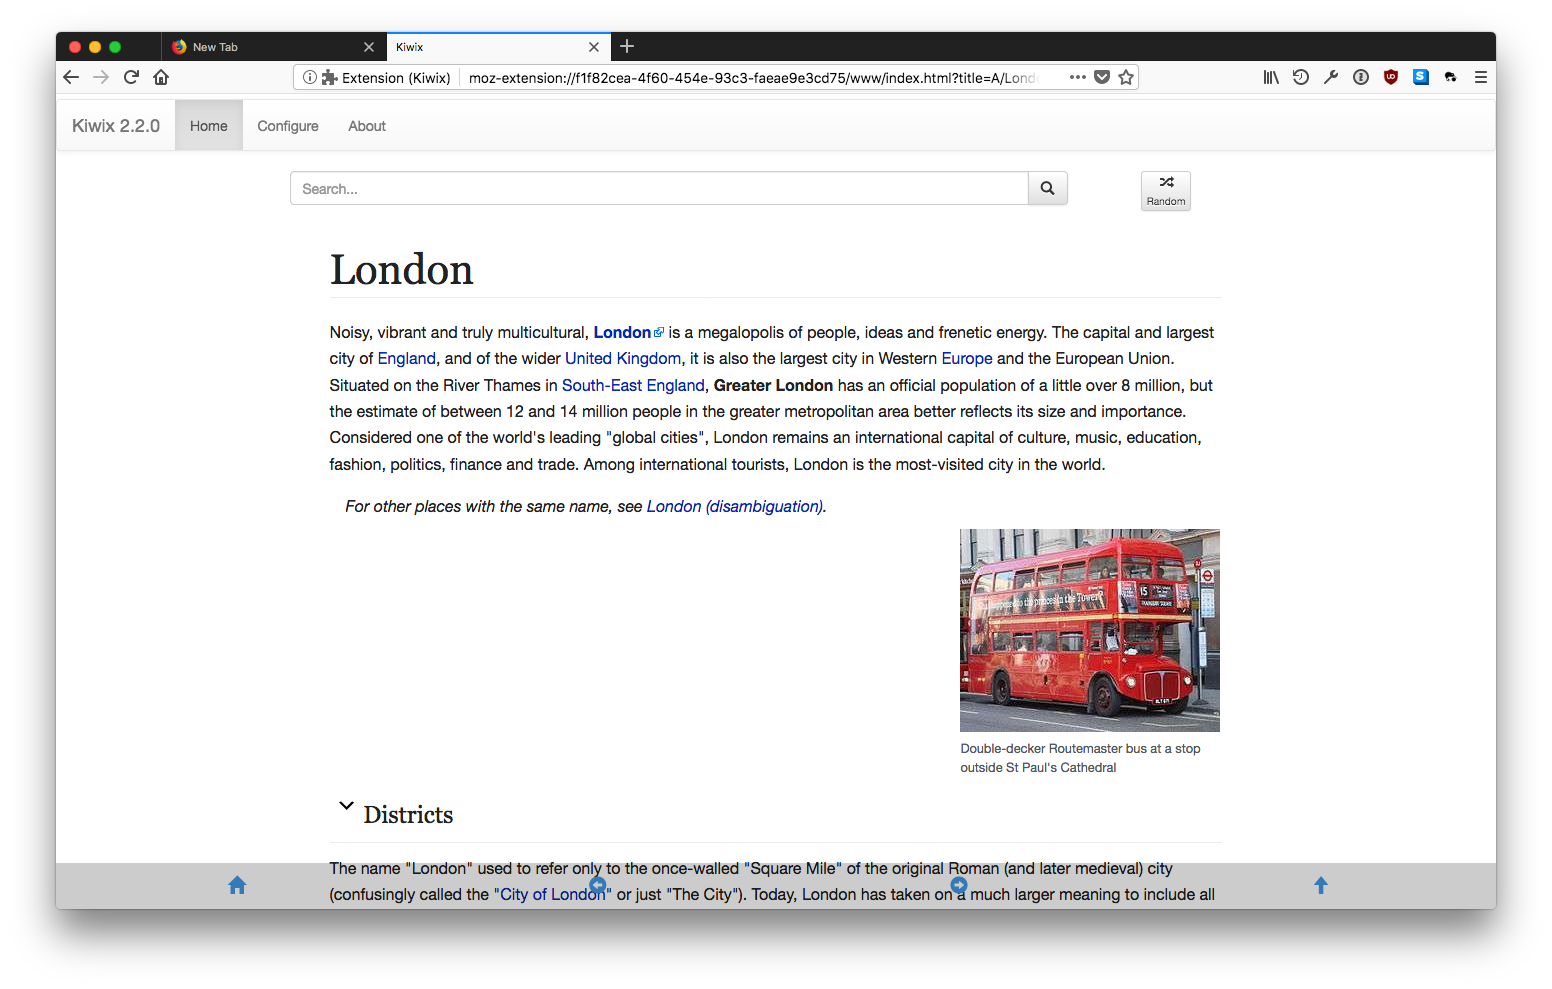
\includegraphics[width=\textwidth]{images/kiwix-js-extension}
		\caption{Kiwix-JS running in FireFox}
		\label{fig:kiwix-firefox}
	\end{center}
\end{figure}

Kiwix JS as it stands has support for Wikimedia and StackOverflow ZIM files (although others may work, just not supported). This meant that if I could get SAFE Wiki working then it would be possible to not only browse Wikimedia content but also content coming from StackOverflow. The content that users could browse on the SAFE Network would be static, but with that comes some benefits.

\section{Static versus Dynamic Content}

When the idea to 'build a Wikipedia on the SAFE Network' first came to mind, I was very well aware of the fact that most likely nobody would use it. It would exist as nothing more than a tech demo with the slight hope that I would be able to continue developing it after I had finished my studies. Getting enough users to start contributing content, and building an environment where strict moderation could occur, would have been a fools-errand. Especially in the time permissible for this project. I just wouldn't have been able to build a full Wiki system on the SAFE Network and do it justice.

It is with that realisation that I came to discover Kiwix. Instead of trying to build a Wiki system on the SAFE Network and trying to bring users across, why not bring Wikipedia (and other sites) to the SAFE Network. This wouldn't be dynamic in anyway (in that users can edit the content) but it would be there for consumption. The storage of the data facilitated by all the features that the SAFE Network has to offer. An important thing about this approach is that by the end of the year I could have a working and browsable copy Wikipedia on the SAFE Network. In its entirety. Not just a simple throwaway tech demo, but a tool that people might actually be able to use.

Websites like Wikipedia only work because of their user base. When a user edits an article this change is logged and anyone can review any changes made. As there are thousands of users anything that is grievously wrong is likely to be flagged and addressed quickly. Similarly if someone is acting as a \textit{bad-party} and editing pages wrongfully (think governments editing pages of staff members to make them appear in a better light) can be blocked based on IP address. This simple measure means that, in most cases, edits are tied to an IP address and hence can be blocked. A simple example is a school, I don't think it needs explaining that school children can be known for being rather silly sometimes. Resulting in the vandalism of some Wikipedia pages. As this is the case it is trivial for Wikipedia to block the IP address(s) that belongs to a school (from making edits) and prevent any further vandalism. On the SAFE Network, this approach is impossible. A user could simply create another account and vandalise an open wiki all they want. It is for reasons such as the ones outlined above that building a dynamic wiki (with adequate moderation techniques/tools) would have been very difficult and most likely a fools errand with the time I have allotted for this project. A static Wiki however, was very achievable.

A static version of Wikipedia might at first seam quite rigid, but in the context of the SAFE Network it makes sense. As the network has a concept of \textit{ownership of data}, a ZIM file that has been uploaded can be directly tied to an account. The ZIM file belongs to someone (an account) in a verifiable \textit{cryptographic} manner. An organisation like Wikimedia, or a trusted third-party, can then upload ZIM files to the network with the assurance that users will know it came from them. It will then exist on the network as an un-censorable mirror (or archive) of whatever source the ZIM file came from. Everyone that has access to the SAFE Network can access it, the only person that is allowed to modify (delete) the file is the holder of the account used to upload the file. As long as you trust the source of the ZIM file, you can \textit{trust} that the information contained within it came from them.

The combination of Kiwix and the SAFE Network makes total sense within this context. A strong pedigree, and the foundation to read and process the ZIM files (static content), meant I could build a tool that could be useful to many people around the world.

\section{Electron}

Electron allows you to "Build cross platform desktop apps with JavaScript, HTML, and CSS". Being able to produce an application that was cross platform was very important to me. The SAFE Network is not platform specific so SAFE Wiki shouldn't be either. As Kiwix JS is built upon web-technologies, Electron seamed like the obvious answer as to how to pull Kiwix JS outside of the web browser environment. Under the hood, Electron combines \textit{Node.js} and \textit{Chromium} into a single environment that can be deployed to the three main platforms: Windows, Linux and macOS. As there exists a \textit{Node.js API} for the SAFE Network this meant that a single application could be built. A single application that could handle both the uploading and deletion of ZIM files on the network and also the browsing of them. The decision not to use the \textit{Web API} to make SAFE Wiki was born out of the requirement of file uploading. To facilitate the upload of large files, (The ZIM for Wikipedia with images is \textgreater 70GB) I really needed to build a desktop application. 

Electron, and indeed Javascript, was very much a new world to me. Beyond simple web development I really haven't done anything note worthy in Javascript. Making Kiwix JS run as an Electron application was hence quite a challenge. After a couple of months of work though I managed to get it running. It was a case of 'completely broken' then one fix lead to 'completely working'. What was now SAFE Wiki, could browse ZIM files from local storage and maintained all the functionality of Kiwix JS.

\printbibliography

\end{document}
